\textbf{Beispiel 4}\\
a)\\ \\
Die Normalvektoren lauten
\[
	\textbf{n}_1 = -\textbf{e}_z \quad \textbf{n}_2 = \textbf{e}_z \quad \textbf{n}_ = \cos(\varphi)\textbf{e}_r -\sin(\varphi)\textbf{e}_z
\]
b) \\ \\
Die konvektive Wärmestromdichte lautet
\[
	\dot{q}_c(z) = \alpha_c(T(t,z) - T\infty)\textbf{n}_3
\]
\newpage
\noindent
c) \\ \\
Die drei gesuchten Wärmeströme lauten
\begin{align*}
	\dot{Q}_1 &= \dot{q}(z')r^2(z')\pi \\
	\dot{Q}_2 &= -\dot{q}(z'')r^2(z'')\pi \\
	\dot{Q}_3 &= -\int_{z'}^{z''}2\pi r(z)\alpha_c(T(t,z) - T_\infty)\frac{1}{\cos(\alpha)}\text{d}z
\end{align*}
d)\\ \\
Die Energiebilanz für das gegebene Kontrollvolumen lautet
\[
	\int_{z'}^{z''}\rho c_p\frac{\partial T(t,z)}{\partial t}\pi r^2(z) - \frac{\partial}{\partial z}(r^2(z)\pi\lambda\frac{\partial T(t,z)}{\partial z}) + 2\pi r(z)\alpha_c(T(t,z) - T_\infty)\frac{1}{\cos(\alpha)}\text{d}z = 0
\]
e)\\ \\
Die Integration muss für jedes $z'$ und $z''$ erfüllt sein. Daher muss die Bedingung aus der Angabe erfüllt sein.\\ \\
f)\\ \\
Die RC-Ersatzschaltung lautet
\begin{figure}[h]
	\centering
	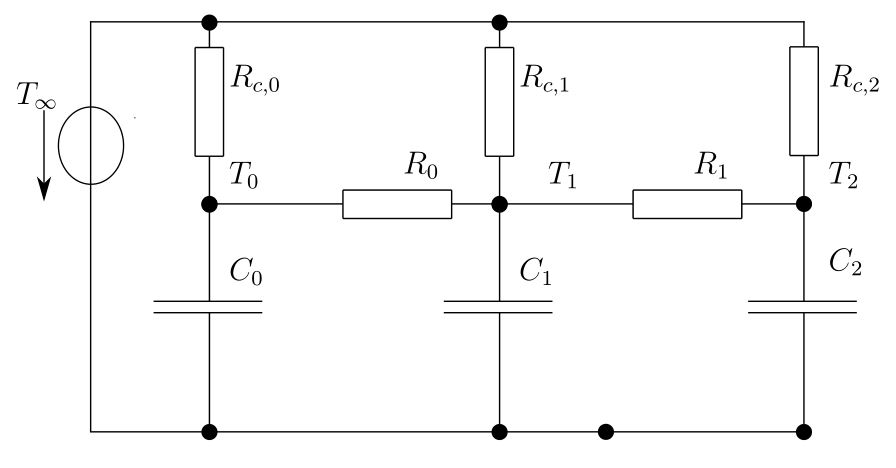
\includegraphics[width= 10cm]{tikz/30_11_2018_4f}
\end{figure}